\begin{frame}[fragile]
    \frametitle{Architecture}
    \begin{figure}
        \resizebox{.9\linewidth}{!}{
            \newlength{\moduledistance}
\setlength{\moduledistance}{1cm}
\overfullrule=2cm
\tikzset{
    module/.style={
           rectangle,
%           rounded corners,
           draw=mDarkTeal, very thick,
           minimum width=3cm,
           minimum height = 0.7cm,
           node distance = 1.5cm,
           inner sep=2pt,
           text centered,
           },
}

\tikzset{
    core/.style={
           circle,
           draw=mDarkTeal, very thick,
           minimum width=2cm,
           inner sep=2pt,
           text centered,
           },
}

\tikzset{
    arrow/.style={
           ->,
           draw=mDarkTeal, very thick,
    }
}

\tikzset{
    darrow/.style={
           <->,
           draw=mDarkTeal, very thick,
    }
}

\begin{tikzpicture}[->,>=stealth']
    \node[core] (core) {
        Core
    };
    \node[module,
          right of=core,
          right=\moduledistance,
          ] (grammatical) {
          Grammatical
    };
    \node[module,
          below of=grammatical,
          ] (standalone) {
        \begin{tabular}{c}
        Machine Learning\\Standalone
        \end{tabular}
    };
    \node[module,
          above of=grammatical,
          ] (reformulation) {
        \begin{tabular}{c}
        Machine Learning\\Reformulation
        \end{tabular}
    };
    \node[module,
          left of=core,
          left=\moduledistance,
          ] (wikidata) {
        Wikidata
    };
    \node[module,
          above of=wikidata,
          ] (cas) {
        Computer Algebra
    };
    \node[module,
          below of=wikidata,
          ] (spellchecker) {
        Spell-checker
    };
    \node[module,
          above of=core,
          above=1cm,
          ] (webui) {
        \begin{tabular}{c}
        Web User\\
        Interface
        \end{tabular}
    };
    \node[module,
          above of=reformulation,
%          right=\moduledistance,
          ] (logging) {
        Logging backend
    };
    \draw[mLightBrown,thick] ($(reformulation.north west)+(-0.3,0.3)$)  rectangle node[yshift=-2.5cm,below] {Question Parsing} ($(standalone.south east)+(0.3,-0.3)$);
    \draw[mLightBrown,thick] ($(cas.north west)+(-0.3,0.3)$)  rectangle node[yshift=-2.5cm,below] {Other modules} ($(spellchecker.south east)+(0.3,-0.3)$);

    \draw [darrow] (core)          -- node{} (cas.south east);
    \draw [darrow] (core)          -- node{} (wikidata.east);
    \draw [darrow] (core)          -- node{} (spellchecker.north east);
    \draw [darrow] (core)          -- node{} (reformulation.south west);
    \draw [darrow] (core)          -- node{} (grammatical.west);
    \draw [darrow] (core)          -- node{} (standalone.north west);
    \draw [darrow] (core)          -- node{} (webui.south);
    \draw [darrow] (webui)         -- node{} (logging.west);
    \draw [arrow]  (logging)       -- node{} (reformulation.north);
    \draw [arrow]  (grammatical)   -- node{} (reformulation.south);

\end{tikzpicture}

        }
    \end{figure}
\end{frame}

\begin{frame}[fragile]
    \frametitle{Datamodel}
    How to represent formally a question asked in natural language?

    \alert{Tree} structure.
\end{frame}
\begin{frame}[fragile]
    \frametitle{Datamodel \--- Leaves: resources}
        \begin{itemize}
            \item Strings: "Isaac \textsc{Newton}"
            \item Dates: 25 December 1642
            \item Geographic coordinates: 47° 30' 18'' N ; 9° 44' 57'' E
            \item \ldots
        \end{itemize}
\end{frame}
\begin{frame}[fragile]
    \frametitle{Datamodel \--- Nodes: operations}
        \begin{itemize}
            \item Full \alert{triples}: (Isaac \textsc{Newton}, birth date, 25 December 1642 (Julian)) $\rightarrow$ true
            \item Missing: (?, birth date, 25 December 1642 (Julian)) $\rightarrow$ [Isaac \textsc{Newton}]
            \item Union, Intersection, Difference, \ldots
            \item And, Or, Not
            \item Exists
            \item Sort, First, Last
        \end{itemize}
\end{frame}

\begin{frame}[fragile]
    \frametitle{Datamodel \--- Examples}
        \only<1>{          
        \begin{center}
        \alert{"Is Brussels the capital of Belgium and the European Union?"}
        \begin{figure}
          \resizebox{\linewidth}{!}{
            \begin{tikzpicture}
              \node (0) at (10,8.5) {$\bigwedge$};
              \node (1) at (7,7) {$\triple$};
              \node (11) at (5,5.5) {Belgium};
              \node (12) at (7,5.5) {capital};
              \node (13) at (8.5,5.5) {Brussels};
              
              \node (2) at (13,7) {$\triple$};
              \node (21) at (11,5.5) {European Union};
              \node (22) at (13,5.5) {capital};
              \node (23) at (15,5.5) {Brussels};

              \node (9) at (14,1) {}; % utilisé pour forcer le positionnement de la figure globale

              \draw[->, >=latex] (0) edge node[sloped, anchor=center, above] {} (1);
              \draw[->, >=latex] (1) edge node[sloped, anchor=center, above] {\scriptsize{subj.}} (11);
              \draw[->, >=latex] (1) edge node[sloped, anchor=center, above] {\scriptsize{pred.}} (12);
              \draw[->, >=latex] (1) edge node[sloped, anchor=center, above] {\scriptsize{obj.}} (13);
              \draw[->, >=latex] (0) edge node[sloped, anchor=center, above] {} (2);
              \draw[->, >=latex] (2) edge node[sloped, anchor=center, above] {\scriptsize{subj.}} (21);
              \draw[->, >=latex] (2) edge node[sloped, anchor=center, above] {\scriptsize{pred.}} (22);
              \draw[->, >=latex] (2) edge node[sloped, anchor=center, above] {\scriptsize{obj.}} (23);
             \end{tikzpicture}
            }
            \end{figure}

          \end{center}}
            
        \only<2>{
          \begin{center}
            \alert{"Who is the mayor of the capital of Kreis Bergstraße?"}
            \begin{figure}
                 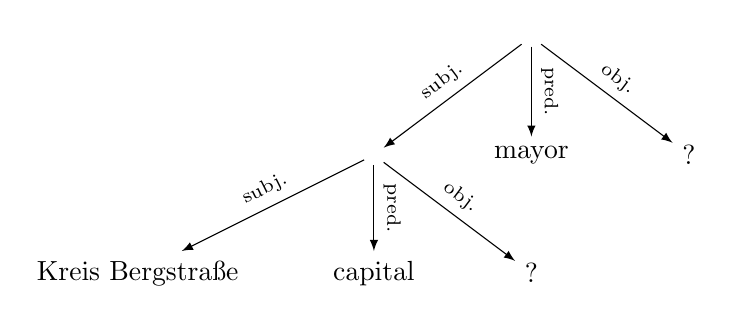
\begin{tikzpicture}
                  \node (0) at (10,10) {$\triple$};
                  \node (1) at (10,8.5) {mayor};
                  \node (2) at (12,8.5) {?};
                  \node (3) at (8,8.5) {$\triple$};
                  \node (4) at (8,7) {capital};
                  \node (5) at (5,7) {Kreis Bergstraße};
                  \node (6) at (10,7) {?};

                  \draw[->, >=latex] (0) edge node[sloped, anchor=center, above] {\scriptsize{obj.}} (2);
                  \draw[->, >=latex] (0) edge node[sloped, anchor=center, above] {\scriptsize{pred.}} (1);
                  \draw[->, >=latex] (0) edge node[sloped, anchor=center, above] {\scriptsize{subj.}} (3);
                  \draw[->, >=latex] (3) edge node[sloped, anchor=center, above] {\scriptsize{subj.}} (5);
                  \draw[->, >=latex] (3) edge node[sloped, anchor=center, above] {\scriptsize{obj.}} (6);
                  \draw[->, >=latex] (3) edge node[sloped, anchor=center, above] {\scriptsize{pred.}} (4);
                 \end{tikzpicture}
                \end{figure}
          \end{center}}
            
        \only<3>{
         \begin{center}
            \alert{"What is the birth date of the first president of Germany?"}
            \begin{figure}
                 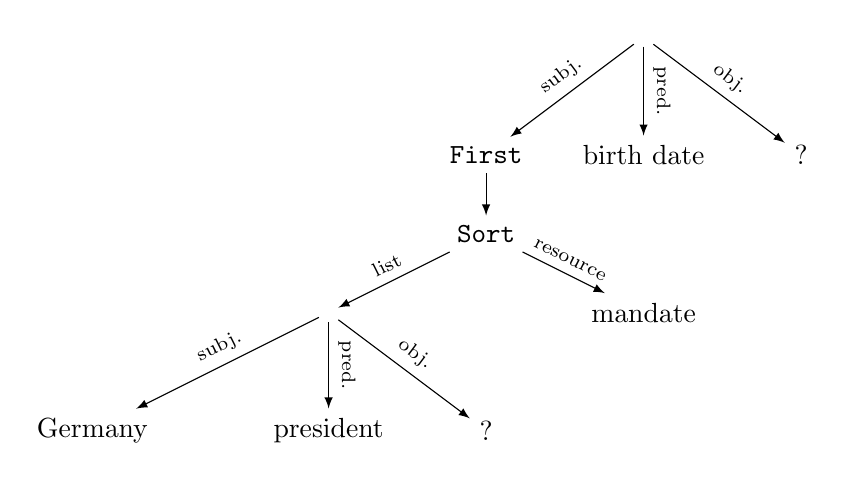
\begin{tikzpicture}
                  \node (0) at (10,10) {$\triple$};
                  \node (1) at (10,8.5) {birth date};
                  \node (2) at (12,8.5) {?};
                  \node (8) at (8,8.5) {\texttt{First}};
                  \node (9) at (8,7.5) {\texttt{Sort}};
                  \node (10) at (10,6.5) {mandate};
                  \node (3) at (6,6.5) {$\triple$};
                  \node (4) at (6,5) {president};
                  \node (5) at (3,5) {Germany};
                  \node (6) at (8,5) {?};

                  \draw[->, >=latex] (0) edge node[sloped, anchor=center, above] {\scriptsize{obj.}} (2);
                  \draw[->, >=latex] (0) edge node[sloped, anchor=center, above] {\scriptsize{pred.}} (1);
                  \draw[->, >=latex] (0) edge node[sloped, anchor=center, above] {\scriptsize{subj.}} (8);
                  \draw[->, >=latex] (8) edge node[sloped, anchor=center, above] {} (9);
                  \draw[->, >=latex] (9) edge node[sloped, anchor=center, above] {\scriptsize{resource}} (10);
                  \draw[->, >=latex] (9) edge node[sloped, anchor=center, above] {\scriptsize{list}} (3);
                  \draw[->, >=latex] (3) edge node[sloped, anchor=center, above] {\scriptsize{subj.}} (5);
                  \draw[->, >=latex] (3) edge node[sloped, anchor=center, above] {\scriptsize{obj.}} (6);
                  \draw[->, >=latex] (3) edge node[sloped, anchor=center, above] {\scriptsize{pred.}} (4);
                 \end{tikzpicture}
                \end{figure}
          \end{center}}

        \only<4>{
          \begin{center}
            \alert{"Is there a medical treatment for Ebola?"}
            \medbreak
            \begin{figure}
                \begin{tikzpicture}
                  \node (0) at (10,8.5) {\texttt{Exists}};
                  \node (1) at (10,7) {$\triple$};
                  \node (11) at (7.5,5.5) {Ebola};
                  \node (12) at (10,5.5) {medical treatment};
                  \node (13) at (12,5.5) {?};

                  \node (9) at (14,1) {}; % utilisé pour forcer le positionnement de la figure globale

                  \draw[->, >=latex] (0) edge node[sloped, anchor=center, above] {} (1);
                  \draw[->, >=latex] (1) edge node[sloped, anchor=center, above] {\scriptsize{subj.}} (11);
                  \draw[->, >=latex] (1) edge node[sloped, anchor=center, above] {\scriptsize{pred.}} (12);
                  \draw[->, >=latex] (1) edge node[sloped, anchor=center, above] {\scriptsize{obj.}} (13);
                 \end{tikzpicture}
                \end{figure}
            \end{center}}

        \only<5>{
          \begin{center}
            \alert{"Who are the children of François \textsc{Mitterrand} and Anne \textsc{Pingeot}?"}
            \begin{figure}
              \resizebox{\linewidth}{!}{
                \begin{tikzpicture}
                  \node (0) at (10,8.5) {$\bigcap$};
                  \node (1) at (7,7) {$\triple$};
                  \node (11) at (4.5,5.5) {François \textsc{Mitterrand}};
                  \node (12) at (7,5.5) {child};
                  \node (13) at (9,5.5) {?};
                  
                  \node (2) at (13,7) {$\triple$};
                  \node (21) at (11,5.5) {Anne \textsc{Pingeot}};
                  \node (22) at (13,5.5) {child};
                  \node (23) at (15,5.5) {?};

                  \node (9) at (14,1) {}; % utilisé pour forcer le positionnement de la figure globale

                  \draw[->, >=latex] (0) edge node[sloped, anchor=center, above] {} (1);
                  \draw[->, >=latex] (1) edge node[sloped, anchor=center, above] {\scriptsize{subj.}} (11);
                  \draw[->, >=latex] (1) edge node[sloped, anchor=center, above] {\scriptsize{pred.}} (12);
                  \draw[->, >=latex] (1) edge node[sloped, anchor=center, above] {\scriptsize{obj.}} (13);
                  \draw[->, >=latex] (0) edge node[sloped, anchor=center, above] {} (2);
                  \draw[->, >=latex] (2) edge node[sloped, anchor=center, above] {\scriptsize{subj.}} (21);
                  \draw[->, >=latex] (2) edge node[sloped, anchor=center, above] {\scriptsize{pred.}} (22);
                  \draw[->, >=latex] (2) edge node[sloped, anchor=center, above] {\scriptsize{obj.}} (23);
                 \end{tikzpicture}
                }
                \end{figure}
            \end{center}}

\end{frame}
